%%%%%%%%%%%%%%%%%%%%%%%%%%%%%%%%%%%%%%%%%%%%%%%%%%%%%%%%%%%%%%%%%%%%%%%%%%%%%%

%%%%%%%%%%%%%%%%%%%%%%%%%%%%%%%%%%%%%%%%%%%%%%%%%%%%%%%%%%%%%%%%%%%%%%%%%%%%%%
\section{Fabrication Methods}

Fabrication follows a layer-by-layer process in which each functional layer is deposited after the previous layer has been completed and inspected. Shadow masks define the metallic and semiconducting layers, whereas the dielectric layers cover the full device area. The main fabrication steps are physical vapor deposition (PVD), chemical vapor deposition (CVD), and spin coating.

%%%%%%%%%%%%%%%%%%%%%%%%%%%%%%%%%%%%%%%%%%%%%%%%%%%%%%%%%%%%%%%%%%%%%%%%%%%%%%
\subsection{Physical Vapor Deposition}

\begin{figure}[h]
\centering
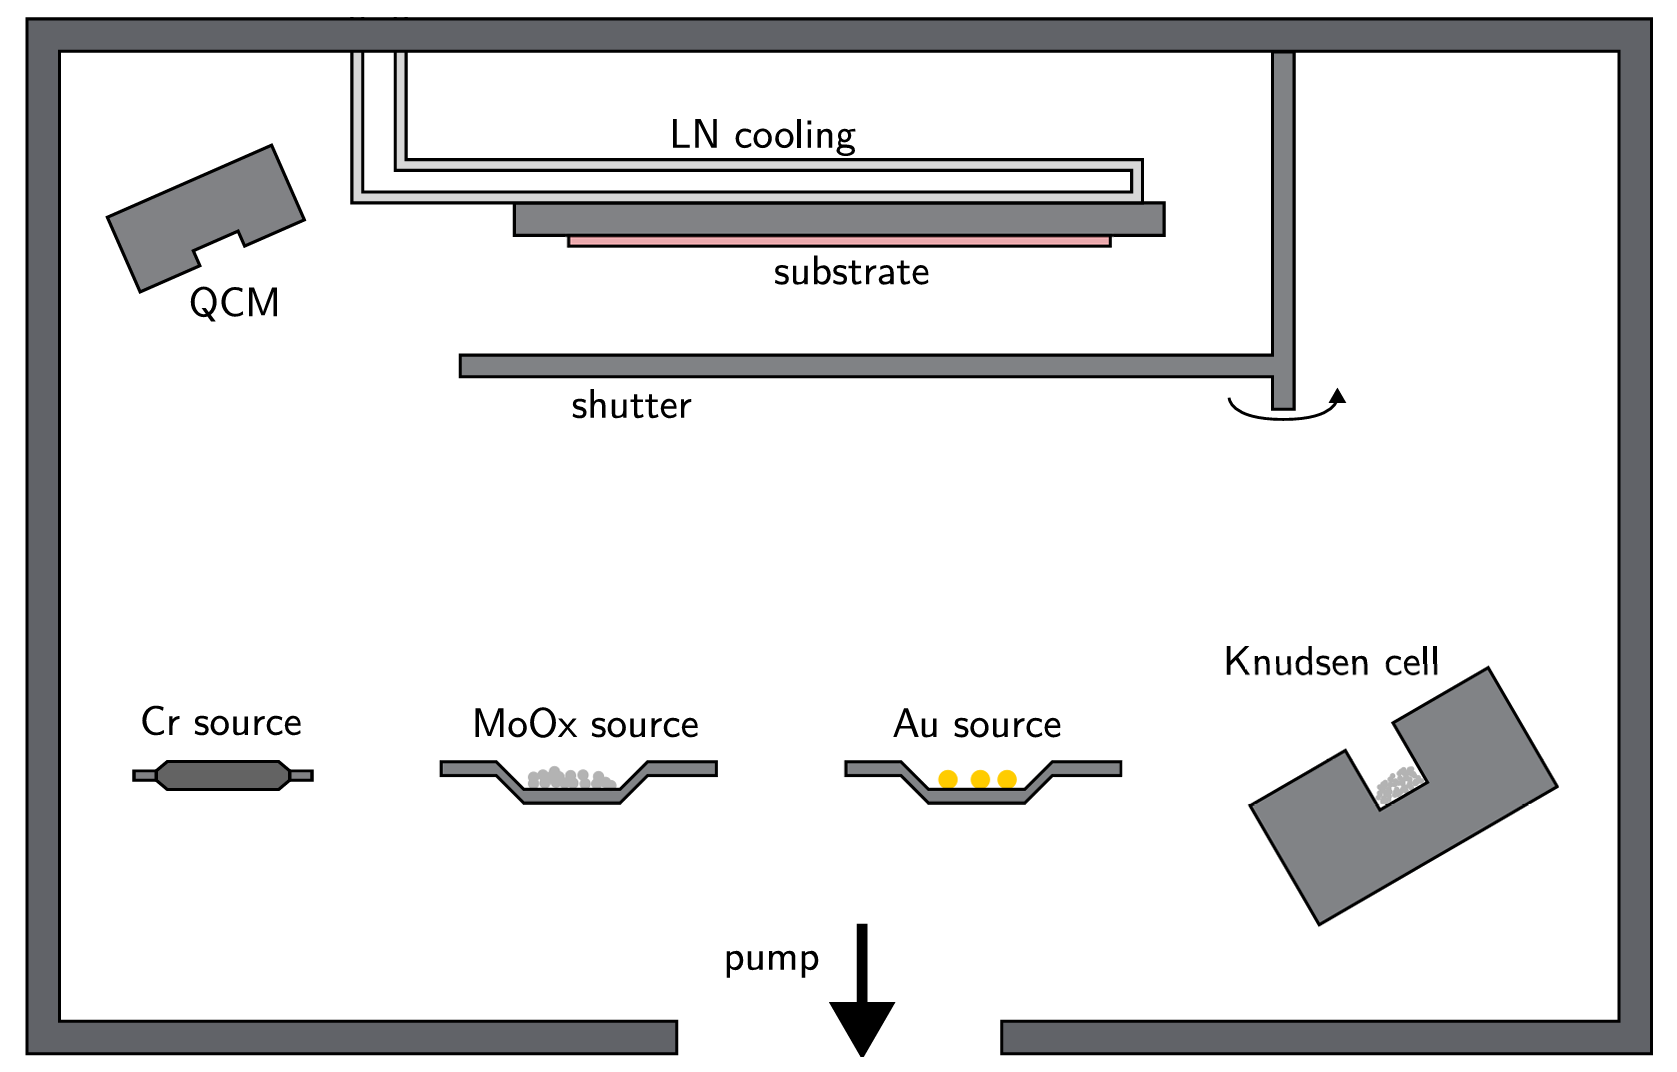
\includegraphics[width=0.65\textwidth]{figures/PVD-layout.png}
\caption[Schematic of the physical vapor deposition system]{Schematic of the physical vapor deposition (PVD) system. Figure from Ref.~\cite{Riederer2023Dissertation}.}
\label{fig:pvd_layout}
\end{figure}

Physical vapor deposition is used for the metallic layers and for the molecular semiconductor. The samples and shadow mask are mounted in the substrate holder, while the source material is placed in the lower part of the vacuum chamber. Metals are heated until they evaporate, and the organic semiconductor is typically evaporated from a Knudsen cell. The evaporated material then travels through the chamber and condenses on the sample surface.

Deposition is performed under high-vacuum conditions to reduce contamination by residual gas molecules and to make the particle mean free path larger than the chamber dimensions. The particles can therefore travel approximately ballistically from the source to the substrate, which is important because shadow-mask patterns are defined by the line-of-sight path through the mask openings.

A shutter between source and sample remains closed while the source is heated and possible impurities are removed. Once the deposition rate has stabilized, the shutter is opened and film growth begins. The film thickness is monitored with a quartz-crystal microbalance, and deposition is stopped when the desired thickness is reached.

In the fabricated devices, PVD is used for the Cr gate, the molecular semiconductor, the MoO$_x$/Au injection contacts, and the Cr/Ag/Au contact pads. Careful mask alignment is essential because the injection contacts must overlap the semiconductor while remaining electrically separated from one another.

%%%%%%%%%%%%%%%%%%%%%%%%%%%%%%%%%%%%%%%%%%%%%%%%%%%%%%%%%%%%%%%%%%%%%%%%%%%%%%
\subsection{Chemical Vapor Deposition of Parylene-N}

\begin{figure}[h]
\centering
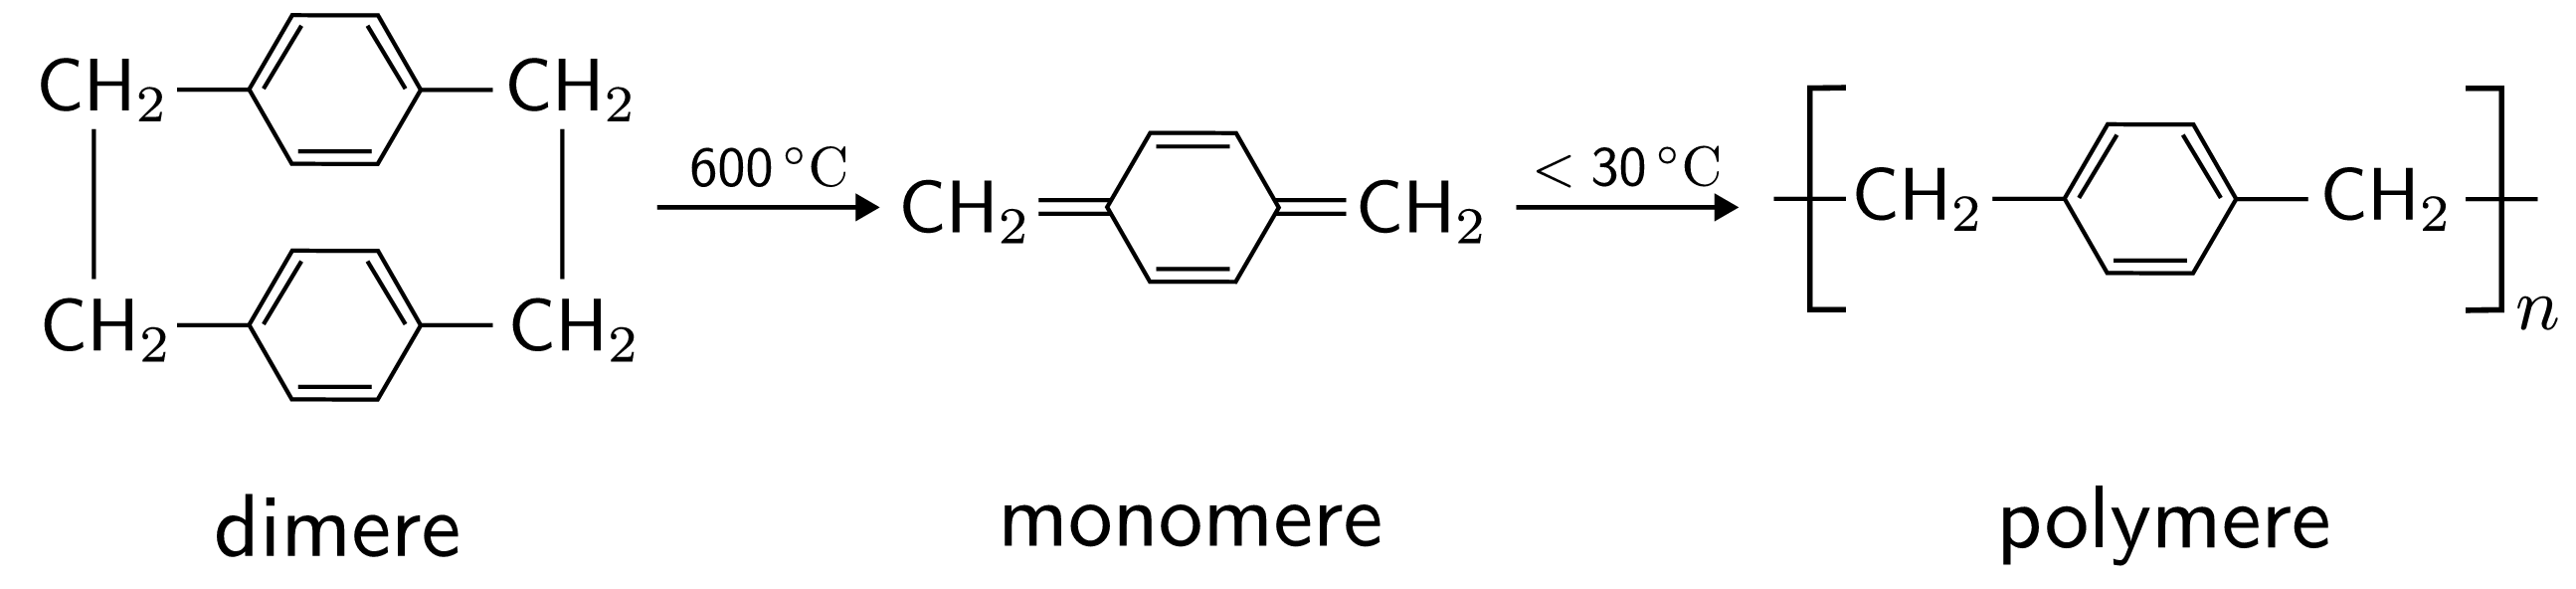
\includegraphics[width=0.65\textwidth]{figures/PaN-CVD.png}
\caption[Schematic of the chemical synthesis of PaN]{Schematic of the chemical synthesis of parylene-N (PaN). Figure from Ref.~\cite{Riederer2023Dissertation}.}
\label{fig:pan_cvd_reaction}
\end{figure}

\begin{figure}[h]
\centering
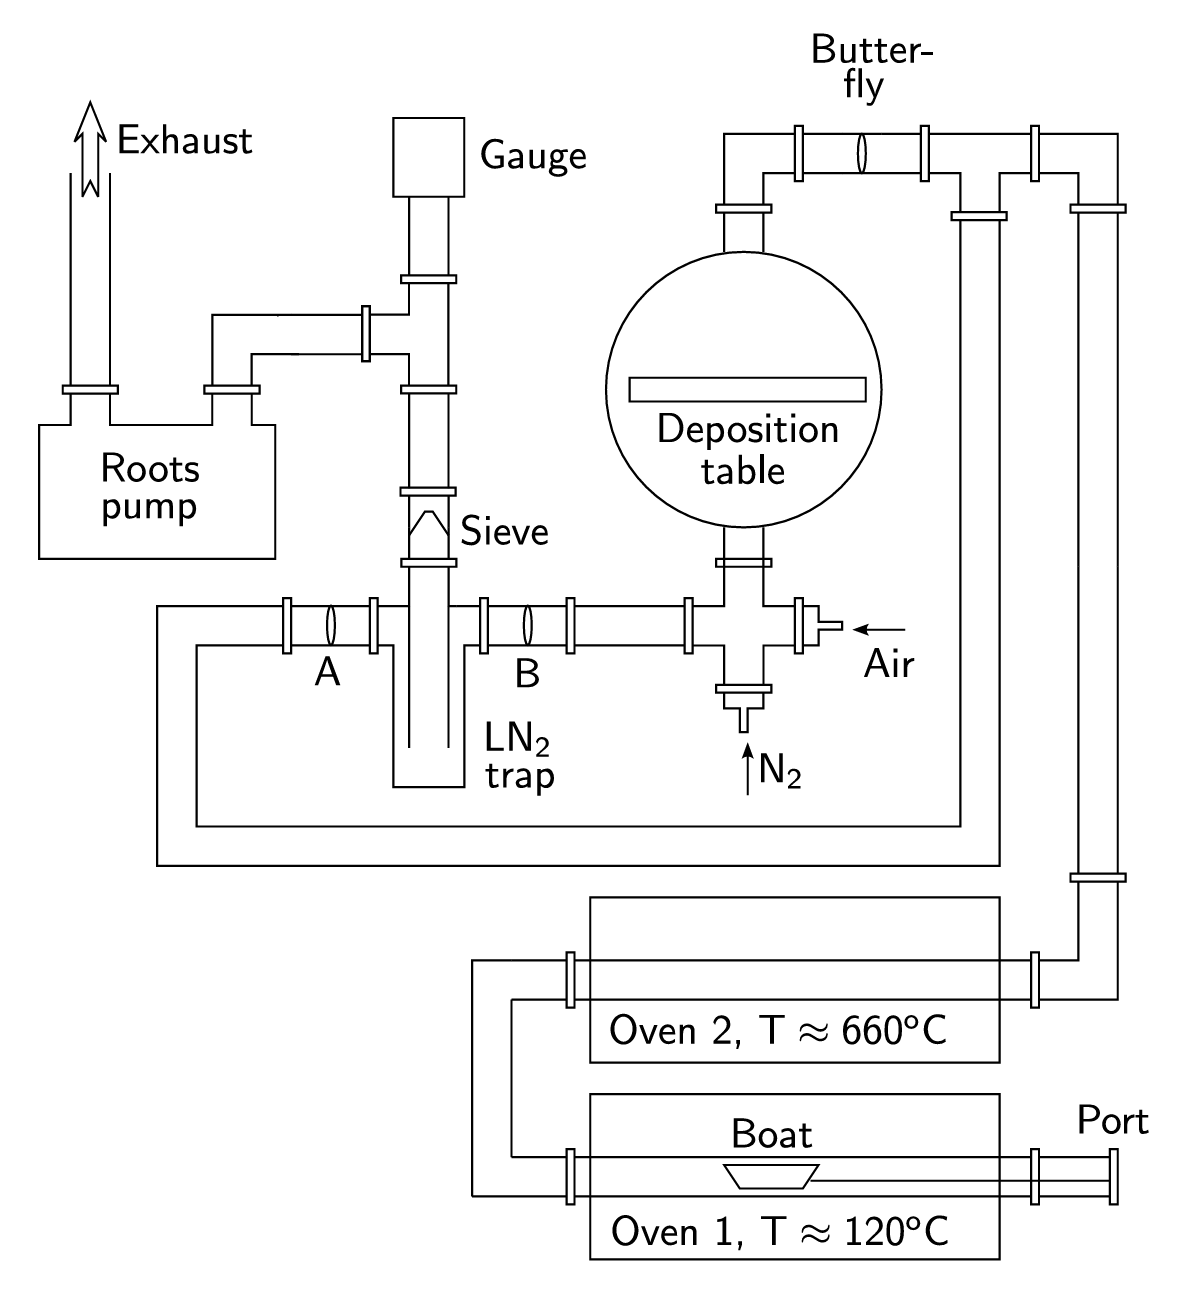
\includegraphics[width=0.6\textwidth]{figures/CVD-layout.png}
\caption[Schematic of the chemical vapor deposition system]{Schematic of the chemical vapor deposition (CVD) system used for PaN deposition. Figure from Ref.~\cite{Kersting2026FiguresCollection}.}
\label{fig:cvd_layout}
\end{figure}

Parylene-N is deposited by chemical vapor deposition. The parylene precursor is first evaporated and then converted into reactive monomers at high temperature. These monomers are transported into the deposition chamber, where they polymerize on the sample surface and form a conformal insulating film.

In the device stack, PaN is the main gate dielectric. It separates the gate electrode from the semiconductor and prevents direct leakage through the gate stack. Gas-phase deposition allows PaN to cover the gate structure uniformly, reducing the risk of pinholes, local thickness variations, leakage, and electrical breakdown.

Before deposition, the system is evacuated and the sample holder can be heated to remove adsorbed water. During deposition, the sample temperature is kept low enough for polymerization on the surface. The target PaN thickness is \SI{300}{\nano\meter}. If the dielectric covers the gate contact areas, they are opened locally before the final contacting step.

%%%%%%%%%%%%%%%%%%%%%%%%%%%%%%%%%%%%%%%%%%%%%%%%%%%%%%%%%%%%%%%%%%%%%%%%%%%%%%
\subsection{Spin Coating of the PS Planarization Layer}

\begin{figure}[h]
\centering
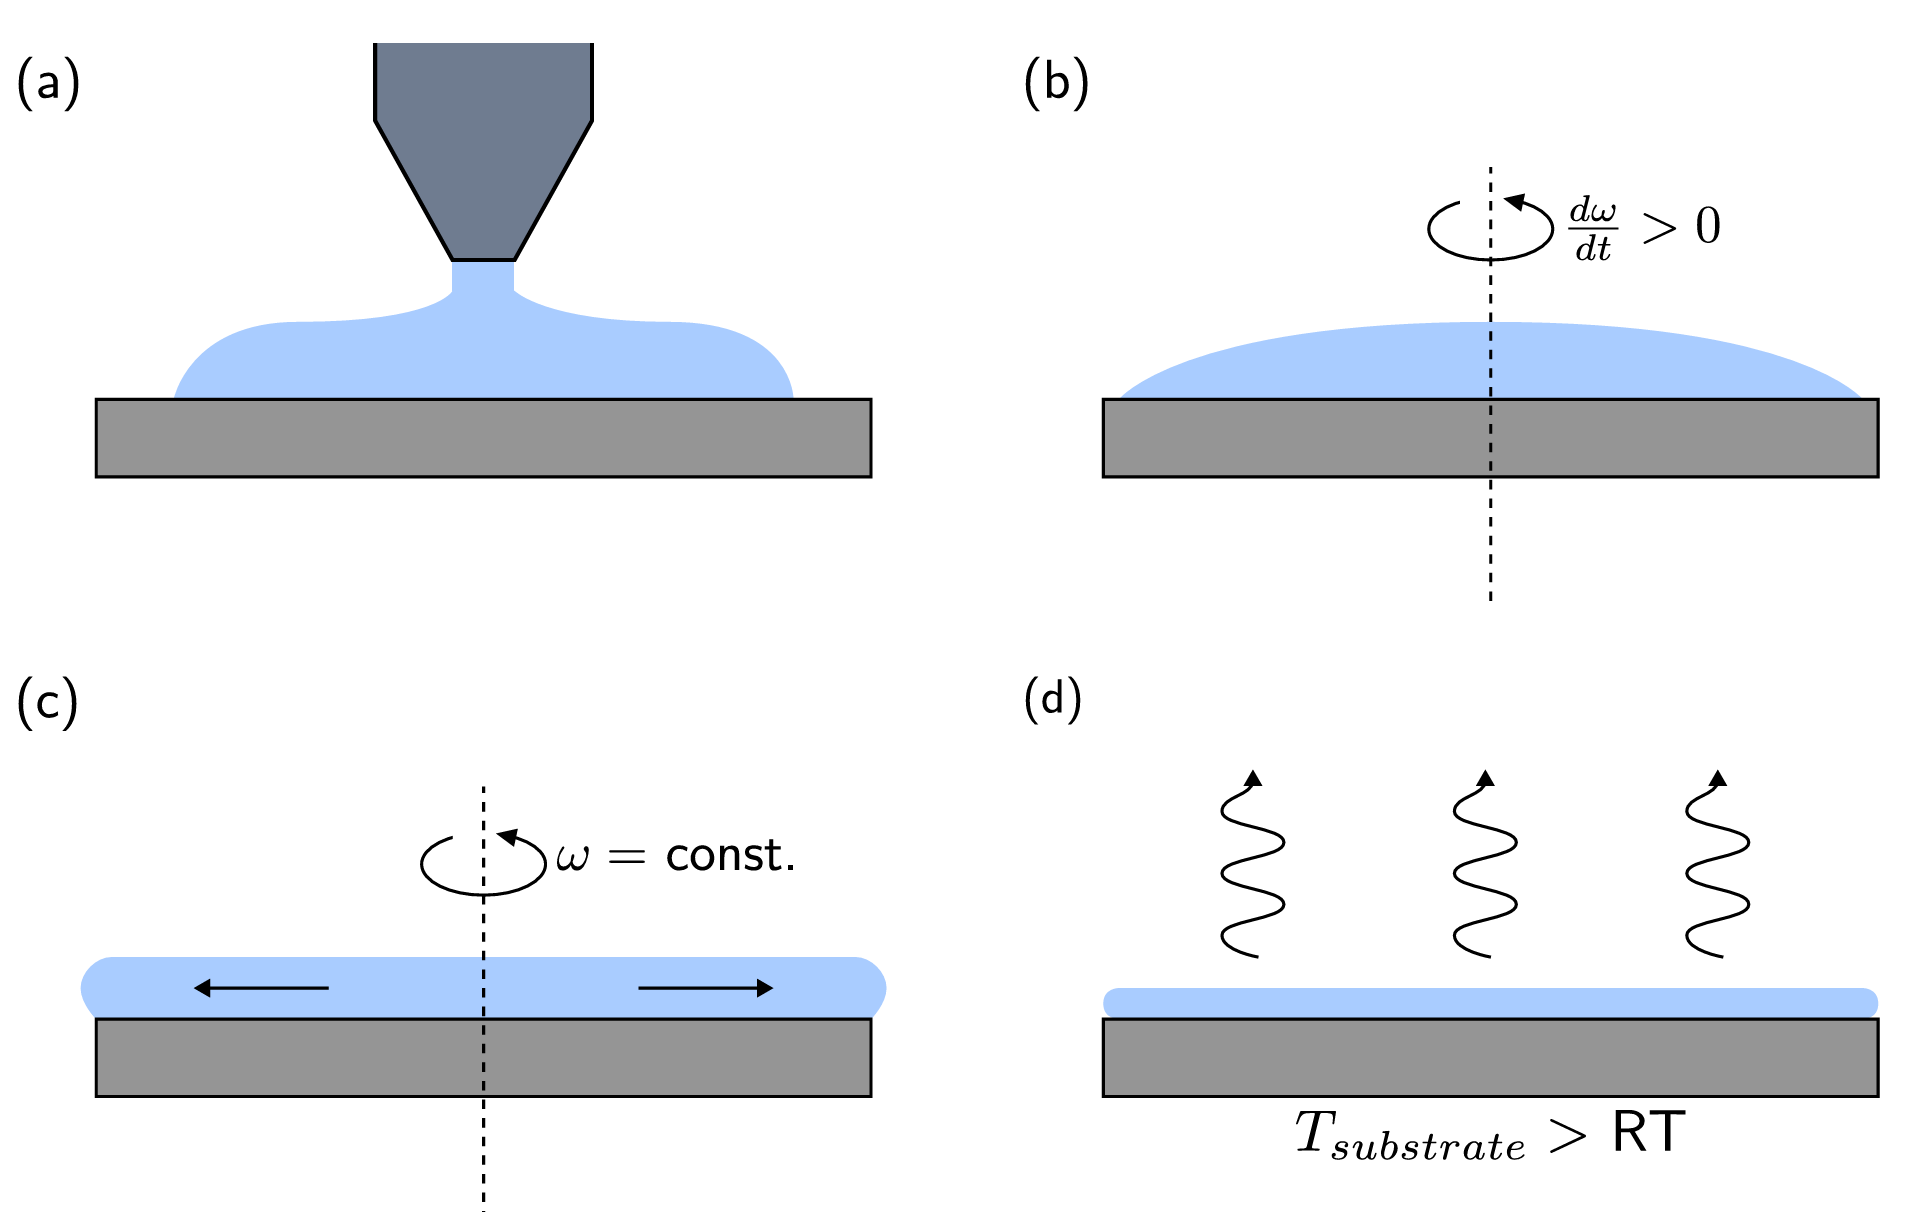
\includegraphics[width=0.60\textwidth]{figures/spincoating-layout.png}
\caption[Schematic of spin coating]{Schematic of the spin coating procedure. Figure from Ref.~\cite{Riederer2023Dissertation}.}
\label{fig:spincoating_layout}
\end{figure}

The PS layer is deposited by spin coating. A polymer solution is dispensed onto the sample, which is then rotated at high speed. Centrifugal forces spread the solution over the surface while solvent evaporates, leaving a thin polymer film. The final thickness depends on the polymer concentration, solvent, spin speed, spin time, and drying conditions.

In this device architecture, PS planarizes the PaN surface and provides a more homogeneous interface for growth of the molecular semiconductor. This is important because molecular ordering and grain formation are sensitive to the dielectric surface. A smoother and chemically more homogeneous surface can improve film reproducibility~\cite{Sirringhaus2005DevicePhysics,Wang2017LowVoltageC8BTBT}.

The target PS thickness is \SI{80}{\nano\meter}. After spin coating, the film is dried to remove residual solvent. The resulting PaN/PS dielectric stack must be continuous and electrically insulating because defects can cause gate leakage and make field-effect measurements unreliable.
